\documentclass{article}

\topmargin 0pt

\topmargin=-1.5cm
\oddsidemargin=0.7cm
\textheight=23.5cm
\textwidth=15cm
\setlength{\baselineskip}{24pt}
\renewcommand{\baselinestretch}{1.5} %行距




\usepackage{fontspec}   %加這個就可以設定字體
\usepackage{xeCJK}       %讓中英文字體分開設置
%\usepackage{times}
\usepackage{amssymb}
\usepackage{amsmath}
\usepackage{amsthm}
\usepackage{ulem}
\usepackage{amsfonts}
\usepackage{mathrsfs}
\usepackage{tabularx,array}
\usepackage{pgf,tikz}
 \usepackage{blkarray} %line 80-92 Q formula matrix index
%\usepackage{colortbl}
\usepackage{enumitem}% enumerate labels   roman
\usepackage{graphicx}
%\usepackage{indentfirst}
\graphicspath{{images/}}
\usetikzlibrary{arrows}
\setCJKmainfont{標楷體} %設定中文為系統上的字型,而英文不去更動,使用原TeX字型
\XeTeXlinebreaklocale "zh"             %這兩行一定要加,中文才能自動換行
\XeTeXlinebreakskip = 0pt plus1pt     %這兩行一定要加,中文才能自動換行
\title{Combinatorial Identities from Lagrange's Interpolation Polynomial}
\author{Student: Yen-Jung Huang  ~~~~~~~~~~~~~~~~~~~~~~~~~~Advisor: Chih-Wen Weng}
\date{} %不要日期

\def\UrlFont{\rm}


\theoremstyle{plain}
\newtheorem{thm}{Theorem}[section]
\newtheorem{cor}[thm]{Corollary}
\newtheorem{lem}[thm]{Lemma}
\newtheorem{prop}[thm]{Proposition}
\newtheorem{remark}[thm]{Remark}
\newtheorem{eg}[thm]{Example}
\newtheorem{conj}[thm]{Conjecture}


\theoremstyle{definition}
\newtheorem{defn}[thm]{Definition}
\newtheorem{ex}[thm]{Exercise}
\newtheorem{prob}[thm]{Problem}
\newtheorem{exam}[thm]{Example}
\newtheorem{nota}[thm]{Notation}
\newtheorem{rem}[thm]{Remark}
\newtheorem{ques}[thm]{Question}
% \newtheorem{pof}[thm]{Proof.}

\usepackage{comment}

%\renewcommand {\refname} {Bibliography}



\begin{document}

%封面

\thispagestyle{empty}
\begin{center}
{ \Huge 國~~~~立~~~~交~~~~通~~~~大~~~~學}~\\~\\

\bigskip

{ \Huge 應~用~數~學~系}~\\~\\

\bigskip

{ \Huge 碩~~士~~論~~文}~\\~\\

\bigskip \bigskip\bigskip\bigskip\bigskip\bigskip

{ \Huge 有向圖譜半徑之簡易估算方法}~\\~\\

\bigskip

{ \Huge A simple method on estimating spectral radius for some direted graphs}~\\~\\
~\\~\\~\\~\\~\\
\bigskip \bigskip\bigskip\bigskip\bigskip\bigskip
\bigskip \bigskip\bigskip\bigskip\bigskip\bigskip
\bigskip\bigskip\bigskip

{ \Large
\begin{tabular}{rcl}
研究生&:&陳科翰\\
指導教授&:&翁志文~教授
\end{tabular} }

\bigskip\bigskip
{ \Large 中~~華~~民~~國~~一~~百~~ㄧ~~十~~年~~一~~月 }
\large
\end{center}
\pagebreak




%%%%%%%%%%%%%%%%%%%%%%%%%%%%%%%%%%%%%%%%%%%%%%%%%%%%%%%%%%%%%%%%%%%%%%%%%
\renewcommand{\baselinestretch}{2} %行距
\thispagestyle{empty}
\begin{center}
{
\Large
有向圖譜半徑之簡易估算方法\\
A simple method on estimating spectral radius for some direted graphs\\~\\
\begin{tabular}{lccr}
Student: Ko-Han Chen  &&~~~& Advisor: Chih-Wen Weng\\
研究生:陳科翰  &&~~~& 指導教授:翁志文~教授
\end{tabular}
}~\\

\bigskip

\renewcommand{\baselinestretch}{1} %行距

{ \LARGE 國~~~~立~~~~交~~~~通~~~~大~~~~學}\\~\\
{ \LARGE 應~用~數~學~系}\\~\\
{ \LARGE 碩~~士~~論~~文}\\~\\~\\~\\~\\
\renewcommand{\baselinestretch}{1} %行距
{ \large A Thesis

Submitted to Department of Applied Mathematics

College of Science

National Chiao Tung University

in Partial Fulfillment of Requirements

for the Degree of Master

in Applied Mathematics
\bigskip \medskip

January 2021

Hsinchu, Taiwan, Republic of China \bigskip \medskip

 中~~華~~民~~國~~一~~百~~ㄧ~~十~~年~~一~~月 }
\end{center}
\pagebreak

\label{abstract}

%中文摘要
\pagenumbering{roman}
\begin{center}
{  \LARGE
有向圖譜半徑之簡易估算方法
\bigskip\bigskip\bigskip

研究生:陳科翰  ~~~~~~~~~~ 指導教授:翁志文~教授 \\
國立交通大學  \\
\bigskip
應用數學系
\bigskip\bigskip\bigskip\bigskip
} \\~\\~\\~\\
\addcontentsline{toc}{section}{Abstract (in Chinese)}
{\large 摘~要}
\end{center}
 \bigskip

 我知道譜半徑是區分圖中點連線關係的重要指標,所以找一個簡單的方法來估算譜半徑
 是很有意義的。一個簡單而且傑出估算譜半徑的方法有一些特徵。首先,誤差被極小化
 ,第二必定存在一個方法正確理性地證明它。列舉這些方法並正確證明會讓這方法穩固
 且可信靠。在估計的領域裡,最好思考過所有的因素,再根據目標,取用估計譜半徑的
 方法,以利之後分析圖的連接矩陣,與其連通性有關的矩陣。
 \\
\bigskip

\noindent 關鍵詞:譜半徑,簡易方法,有向圖,估算。
\pagebreak



%英文摘要
\begin{center}{\LARGE
A simple method on estimating spectral radius for some direted graphs
\bigskip\bigskip\bigskip}

{ \large
Student: Ko-Han Chen  ~~~~~ Advisor: Chih-Wen Weng \\
\Large

Department ~of~ Applied ~Mathematics
\bigskip

National~ Chiao ~Tung~ University
\bigskip\bigskip\bigskip\bigskip}\\
{\large Abstract}
\end{center}

%\begin{abstract}
\addcontentsline{toc}{section}{Abstract (in English)}
I know that spectral radius is an important index to specify the relation of connected vertices in
 the graphs, so it is meanful to find a simple method to estimate spectral readius. A simple and excellent
 executable method to estimate spectral radius has some features. First, the bios is minimized, and second
 there must be a way to prove it sensible. Enumerate these factors and prove it correctly would make this method
 solid and reliable. In the field of estimation, it's better to go through all the factors, and base on one's goal
 to apply the methods of estimating spectral radius before analyzing the adjacency matrix of the graphs, which is
 related to the connectness of the graph.
  
\bigskip


\noindent {\bf Keywords}: spectral radius, simple method, directed graphs, estimation
%\end{abstract}
\pagebreak


\renewcommand{\baselinestretch}{1.2}
% 目錄
\large
\tableofcontents


\pagebreak

\label{Introduction}
% Introduction

\section{Introduction}
\normalsize
\pagenumbering{arabic}

Let $\mathbb{R}$ and $\mathbb{C}$ denote the
 field of real numbers and complex numbers respectively.

\begin{defn}       
Let $C$ be an $n \times n$ real nonnegative matrix, and $u \in \mathbb{R}^n$ be a
 nonzero column vector. The scalar $\lambda \in \mathbb{C}$ is an $\it{eigenvalue}$ 
of C corresponding to the $\it{eigenvector}$ $u,$  if $Cu = \lambda u.$
%Also, $C$ has an left eigenvector $v^T$, when $v^TC=\lambda v^T$.
\end{defn}

\begin{defn} \cite{spec_rad}
    When $C$ is an $n \times n$ real matrix, the $\textit {spectral radius} $ $\rho(C)$
        of $C$ is defined by 
        $$\rho(C):=\max\{~|\lambda|~\ |~~\lambda\hbox{ is an eigenvalue of $C$}\},$$
    where $|\lambda|$ is the magnitude of complex number $\lambda.$
\end{defn}

We are interested in spectral radius of the following matrix associated with a simple graph.

\begin{defn} 
    Given an directed graph G, the$\textit{ adjacency matrix}$ of G is the square 
    matrix $A = (a_{ij})$ indexed by vertices of G, and
     \[a_{ij} =\begin{cases} 
        1, \text{if $i$ is adjacent to $j$}, \\
        0, \text{otherwise.}
            \end{cases}
     \]
\end{defn}

\begin{defn}
    Given a directed graph G, the $\textit{spectral radius}$  $\rho(G) $ of G is the spectral
     radius of the adjacency matrix of G.
\end{defn}

\section{Preliminaries}
    
The next theorem is Perron–Frobenius Theorem, which provides a feature of
 nonnegative eigenvector to nonnegative matrices.
\begin{thm} \cite{chang} \cite{prn_fros2} \label{thm:Perron_Frobenius}
    If $C$ is nonnegative square matrix, then the spectral radius $\rho(C)$ is an
    eigenvalue of $C$ with a corresponding nonnegative right eigenvector and a
    corresponding nonnegative left eigenvector.
\end{thm}

We introduce a notation of submatrix, which is taken from some columns and some rows of a
 matrix.

\begin{defn}
    For a matrix $C=(c_{ij})$ and subsets $\alpha$, $\beta$ of row indices and column 
    indices of $C$ respectively,  We use $C[\alpha|\beta]$ to denote the 
    submatrix of $C$ with size $ |\alpha| \times |\beta| $ that has entries $c_{ij}$ for $i\in \alpha$
    and $j\in\beta$,
\end{defn}


We introduce two matrices $P$ and $Q$ in the following Theorem, where $P$ is a permutation
 matrix which is multiplied to the left side, and $Q$ is sum of elementary matrix and
 certain binary matrix. In which $P$ generalize row permutation on cases of $C$
 matrix,and $Q$ is the transform from $C'$ to C', which is the first n-1 columns
  and sum of certain columns. We aim to find C' such that $C'$ majors $C$,i.e. $C\leq C'$
 
The following Theorem is from \cite{chang}.

\begin{thm}\label{pre_thm}
    Let $C=(c_{ij})$, $C'=(c'_{ij})$, $P$ and $Q$ be  $n\times n$ matrices.
Assume that
\begin{enumerate}[label=(\roman*)]
    \item \label{pre_thm_em1}  $PCQ\leq PC'Q$;
    \item \label{pre_thm_em2} there exist a nonnegative column vector $u=(u_1, u_2, \ldots, u_n)^T$  and a
    scalar $\lambda'\in \mathbb{R}$ such that $\lambda'$ is an eigenvalue of $C'$ with
    associated eigenvector $Qu$;
    \item \label{pre_thm_em3}  there exist a nonnegative row vector $v^T=(v_1, v_2, \ldots, v_n)$  and a scalar
    $\lambda\in \mathbb{R}$such that $\lambda$ is an eigenvalue of $C$ with associated  left
    eigenvector $v^TP$; and
    \item \label{pre_thm_em4} $v^TPQu>0.$
\end{enumerate}
    Then $\lambda\leq \lambda'$. Moreover, $\lambda=\lambda'$ if and only if
    \begin{equation}\label{pre0}
        (PC'Q)_{ij}=(PCQ)_{ij}\qquad \hbox{for~}1\leq i, j\leq n \hbox{~with~} v_i\ne 0 \hbox{~and~} u_j\ne 0.
    \end{equation}
\end{thm}

\begin{proof}
    Multiplying the nonnegative vector $u$ in Theorem~\ref{pre_thm} assumption
    ~\ref{pre_thm_em1}, where $Qu$ is eigenvector of $C'$,  to the right of both terms of
    ~\ref{pre_thm_em1},    
    \begin{equation}\label{pre1}
       PCQu\leq PC'Qu=\lambda'PQu.
    \end{equation}
    Multiplying the nonnegative left eigenvector $v^T$ of $C$ for $\lambda$ in assumption
     ~\ref{pre_thm_em3} to the left of all terms  in (\ref{pre1}), where $v^TP$ is
    left eigenvector of $C$ for $\lambda$, thus we have
    \begin{equation}\label{pre2}
        \lambda v^TPQu=v^TPCQu\leq v^TPC'Qu=\lambda' v^TPQu.
    \end{equation}
        Now delete the positive term $v^TPQu$ by assumption \ref{pre_thm_em4} to obtain
        $\lambda\leq \lambda'$ and finish the proof of the first part.
        Assume that $\lambda=\lambda'$, so the inequality in (\ref{pre2}) is an equality.
        Especially $(PCQu)_i=(PC'Qu)_i$ for any $i$ with $v_i\not=0.$ Hence,
        $(PCQ)_{ij}=(PC'Q)_{ij}$ for any $i$ with $v_i\not=0$ and any $j$ with
        $u_j\not=0.$ Conversely, (\ref{pre0}) implies $$v^TPCQu=\sum_{i,j} v_i(PCQ)_{ij}u_j=
         \sum_{i,j} v_i(PC'Q)_{ij}u_j=v^TPC'Qu,$$ so $\lambda=\lambda'$ by (\ref{pre2}).
\end{proof}

\section{Our Method}
We use $[n-1]$ as notation of the set of elements from one to $n-1$, which is ${1,2,...,n}$.
Throughout fix $k\in [n-1]$.Let $E_{kn}$ denote the $n\times n$ binary matrix with a unique $1$ 
appearing in the position $k,n$ of $E_{kn}$. We will apply the previous Theorem \ref{pre_thm} with $P=I$ and 



\begin{equation} \label{Q_1}
Q=I+E_{kn}=\begin{pmatrix} 
1 &  & & &  & 0 \\
 & 1 &  &      &  &  \\
 &  & \ddots & &  & 1 \\
 &  &        & &  &  \\
  &  & & & 1 &  \\
0 &  & & &  & 1 \\
\end{pmatrix}.  
\end{equation}






\begin{defn}%[$K$-rooted vector]
~A column vector $v'=(v'_1,v'_2,\ldots,v'_n)^T$ is called {\it $K$-rooted}  if $v'_{j} \geq 0$ for $1 \leq  j \leq n$ and $v'_k\geq v'_n.$
\end{defn}
\bigskip

The following Lemma is immediate from the above definition.%[vector rooted lemma]
\bigskip

\begin{lem}\label{lem:rt_vec}
If $u=(u_1, u_2, \ldots, u_n)^T$ and $v'=(v'_1, v'_2, \ldots, v'_n):=Qu=(u_1,\ldots, u_{k-1},u_k+u_n, u_{k+1}, \ldots,  u_n)^T$, then
\begin{enumerate}[label=(\roman*)]
\item \label{lem:rt_vec:en1}$v'$ is $K$-rooted  if and only if  $u$ is nonnegative;
\item $u_k>0$ if and only if $v'_k>v'_n$.
\end{enumerate}
% \qed
\end{lem}

Below is our first result, in which the first condition implies the first n-1 columns of C major to
 the columns of C', and the (k,n)-sum column of C is also major to C'. The second and the third condition
 suggest that C and C' have nonnegative eigenvectors which are k-rooted. And the forth condition is simplier
  but with the same meaning with Theorem (\ref{pre_thm})
\begin{thm}\label{thm_main}
    Let $C=(c_{ij})$, $C'=(c'_{ij})$ be  $n\times n$ matrices.
Assume that
\begin{enumerate}[label=(\roman*)]
\item \label{thm_main:condition_i} $C[[n]|[n-1]]\leq C'[[n]|[n-1]]$ and $c_{ik}+c_{in}\leq c'_{ik}+c'_{in}$ for all $1\leq i\leq n$;
\item \label{thm_main:condition_ii} there exists a $K$-rooted vector $v'=(v'_1, v'_2, \ldots, v'_n)^T$ and a scalar $\lambda'\in \mathbb{R}$
such that $\lambda'$ is an eigenvalue of $C'$ with associated eigenvector $v'$;
\item \label{thm_main:condition_iii}there exists a nonnegative vector $v^T=(v_1, v_2, \ldots, v_n)$ and a scalar $\lambda\in \mathbb{R}$ such that $\lambda$ is an eigenvalue of $C$ with associated left eigenvector $v^T$;
\item \label{thm_main:condition_iv}$v^Tv'>0.$
\end{enumerate}
 Then $\lambda\leq \lambda'$.
Moreover, $\lambda=\lambda'$
if and only if
\begin{enumerate}[label=(\alph*)]
    \item \label{thm_main:equ_cond_a} $c_{ik}+c_{in}=c'_{ik}+c'_{in} \qquad$  for $1\leq i\leq n$ with $v_i\not=0$ and $v'_n\not=0;$
    \item \label{thm_main:equ_cond_b} $c'_{ij}=c_{ij}\qquad $for $1\leq i\leq n,~1\leq j\leq n-1, j \neq k $with $v_i\ne 0 $;
    \item \label{thm_main:equ_cond_c} $c'_{ik}=c_{ik} \qquad $  for $1\leq i \leq n$ and $ v'_{k}>v'_n$ 
\end{enumerate} %\qed
\end{thm}
% 

   
\begin{proof}
    The proof is based on Theorem~\ref{pre_thm} with $P = I$ and $Q = I + E_{kn}$ in (\ref{Q_1}). 
    The assumption \ref{pre_thm_em1} $PCQ\leq PC'Q$ of Theorem~\ref{pre_thm} holds by the condition \ref{thm_main:condition_i} of this Theorem. 
    Let $u = Q^{-1}v'$. Then u is nonnegative and $C'Qu = \lambda' Qu$ by the condition \ref{thm_main:condition_ii} and
     Lemma~\ref{lem:rt_vec}\ref{lem:rt_vec:en1}. Hence the assumption \ref{pre_thm_em2} of Theorem~\ref{pre_thm} holds. The assumptions \ref{pre_thm_em3} and \ref{pre_thm_em4}
      of Theorem~\ref{pre_thm} clearly hold by conditions~\ref{thm_main:condition_iii},\ref{thm_main:condition_iv} of this Theorem since $P = I$ and
       $v'= Qu$  Hence $\lambda \leq \lambda' $ by the necessary condition of Theorem~\ref{pre_thm}. Moreover
        $\lambda = \lambda'$ if and only if \ref{pre0} holds, and this is equivalent to
         conditions \ref{thm_main:equ_cond_a},\ref{thm_main:equ_cond_b},\ref{thm_main:equ_cond_c} of this Theorem. 
\end{proof}   
    
We are interested in the matrices $C'$ that have $K$-rooted eigenvectors.
Motivated by the condition (i) of Theorem 2.3, we provide the following two definitions. 
This is the definition of (k,n)-sum.
\begin{defn}
    For an $n \times n$ matrix $C'=(c'_{ij})$, the $(k, n)$-sum vector of $C'$ is the vector of the sum of the $k$-th and  $n$-th columns of $C'$, where $k\leq n-1$.
\end{defn}

Note that the last column of $C'Q$ is the $(k, n)$-sum vector of $C'$
Below is the definition of k-rooted matrix.
\begin{defn}\label{m_rooted}
    A  matrix $C'=(c'_{ij})$ is called $k-rooted$  if its  columns and its $(k, n)$-sum vector are all $K$-rooted except the last column of $C'$.
\end{defn}


\begin{rem}

    $$Q^{-1}=I-E_{kn}=\begin{pmatrix}
    1 &  & & &  & 0 \\
    & 1 &  &      &  &  \\
    &  & \ddots & &  & -1 \\
    &  &        & &  &  \\
    &  & & & 1 &  \\
    0 &  & & &  & 1 \\
    \end{pmatrix}.$$

    The matrix $C'Q$ is
    $$\begin{pmatrix}
    c'_{11}     & c'_{12} & \cdots     & c'_{1\ n-1} & c'_{1k}+c'_{1n} \\
    \vdots \\
    c'_{k-11}     & c'_{k-1 2}           & \cdots     & c'_{k-1 n-1} & c'_{k-1k}+c'_{k-1n} \\
    c'_{k1} & c'_{k2} &\cdots      & c'_{kn-1} & c'_{kk}+c'_{kn}\\
    c'_{k+11}     & c'_{k+12}           & \cdots     & c'_{k+1\ n-1} & c'_{k+1k}+c'_{k+1n} \\
    \vdots              & \vdots & \ddots              & \vdots & \vdots \\
    c'_{n1}             & c'_{n2} & \cdots             & c'_{n\ n-1} & c'_{nk}+c'_{nn} \\
    \end{pmatrix}.
    $$
\end{rem}

The following Theorem shows that a $K$-rooted matrix has a $K$-rooted eigenvector.
\begin{lem}\label{lma_m_rooted}
    Let $C'=(c'_{ij})$ be an $n\times n$ nonnegative matrix. Then the following (i)-(iii) hold.
        \begin{enumerate}[label=(\roman*)]
            \item \label{lma_m_rooted_cond1} $C'$ is a $K$-rooted matrix, if and only if, $Q^{-1}C'Q$ is nonnegative.
            \item \label{lma_m_rooted_cond2}Assume that $C'$ is $K$-rooted and let $u$ be a nonnegative eigenvector of $Q^{-1}C'Q$
                for $\rho(C')$. Then  $C'$ has a $K$-rooted eigenvector $v'=Qu$ for $\rho(C')$. 
            \item \label{lma_m_rooted_cond3}$\rho(C')$ = $\rho(Q^{-1}C'Q)$
        \end{enumerate}
\end{lem}
  

\begin{comment}


\begin{rem}
        (i) is immediate from Definition~\ref{m_rooted} and the observation that   
        $$Q^{-1}=I-E_{kn}=\begin{pmatrix}
        1 &  & & &  & 0 \\
         & 1 &  &      &  &  \\
         &  & \ddots & &  & -1 \\
         &  &        & &  &  \\
          &  & & & 1 &  \\
        0 &  & & &  & 1 \\
        \end{pmatrix},$$
\end{rem}
\end{comment}   
\begin{proof}
    (i)
    and $Q^{-1}C'Q$ is
    $$\begin{pmatrix}
    c'_{11}     & c'_{12} & \cdots     & c'_{1\ n-1} & c'_{1k}+c'_{1n} \\
    \vdots \\
    c'_{k-11}     & c'_{k-1 2}           & \cdots     & c'_{k-1 n-1} & c'_{k-1k}+c'_{k-1n} \\
    c'_{k1}-c'_{n1} & c'_{k2}-c'_{n2} &\cdots      &c'_{kn-1}-c'_{nk-1}& c'_{kk}+c'_{kn}-c'_{nk}-x'_{nn}\\
    c'_{k+11}     & c'_{k+12}           & \cdots     & c'_{k+1\ n-1} & c'_{k+1k}+c'_{k+1n} \\
    \vdots              & \vdots & \ddots              & \vdots & \vdots \\
    c'_{n1}             & c'_{n2} & \cdots             & c'_{n\ n-1} & c'_{nk}+c'_{nn} \\
    \end{pmatrix}.$$
    (ii)
        By Lemma~\ref{lem:rt_vec} $v'=Qu$ is $K$-rooted.  
        Since $Q^{-1}C'Qu=\rho(C')u$ by the assumption, we have
        $Q^{-1} C' Q u  = Q^{-1} \rho(C') Qu  =\rho(C')u$  \\
        $C'Qu=\rho(C')Qu$.

    (iii)
    Since $C'$ and $Q^{-1}C'Q$ have the same set of eigenvalues, clearly $\rho(C')$ = $\rho(Q^{-1}C'Q)$.

\end{proof}


\begin{lem}\label{l_diag}   %end of label
If a square matrix $C'$ has a rooted eigenvector for $\lambda'$, then $C'+dI$ also has
the same rooted eigenvector for $\lambda'+d,$ where $d$ is a constant and $I$ is the identity matrix with the same size of $C'$.
\end{lem}

\begin{thm}\label{thm:conclusion}
    Let $C$ be an $n\times n$ nonnegative matrix. For $1\leq i \leq n$ and $1\leq j\leq n-1$, choose $c'_{ij}$
    such that $c'_{ij}\geq c_{ij}$ and $c'_{kj}\geq c'_{nj}>0$, and choose $r'_i$ such that $r'_i\geq c_{ik}+c_{in}$, and
    $r'_k \geq r'_n$. Moreover choose $c'_{in}:=r'_i-c'_{ik}$. Then $\rho(C)\leq \rho(C')$, when $C'=(c'_{ij})$.
\end{thm}

\begin{proof}
    These assumptions are necessary that $PCQ \leq PC'Q$ where $P = I$,$Q = I+E_{kn}$. And $C'$ is $K$-rooted,based on Lemma
     (\ref{lma_m_rooted}),\\
    $Q^{-1}C'Q$ = 
    $$\begin{pmatrix}
        c'_{11}     & c'_{12} & \cdots     & c'_{1\ n-1} & c'_{1k}+c'_{1n} \\
        \vdots \\
        c'_{k-11}     & c'_{k-1 2}           & \cdots     & c'_{k-1 n-1} & c'_{k-1k}+c'_{k-1n} \\
        c'_{k1}-c'_{n1} & c'_{k2}-c'_{n2} &\cdots      &c'_{kn-1}-c'_{nk-1}& c'_{kk}+c'_{kn}-c'_{nk}-x'_{nn}\\
        c'_{k+11}     & c'_{k+12}           & \cdots     & c'_{k+1\ n-1} & c'_{k+1k}+c'_{k+1n} \\
        \vdots              & \vdots & \ddots              & \vdots & \vdots \\
        c'_{n1}             & c'_{n2} & \cdots             & c'_{n\ n-1} & c'_{nk}+c'_{nn} \\
    \end{pmatrix}.$$
    $Q^{-1}C'Q \geq 0$ for that $c'_{kj}\geq c'_{nj}>0$ when $1\leq j\leq n-1$ , $c'_{ij}\geq c_{ij}$ where $C$ is nonnegative,
    and the last column $c'_{in}+c'_{ik}=r'_i \geq c_{in}+c_{ik}$ by assumption $r'_i\geq c_{ik}+c_{in}$\\

    For $1\leq i \leq n$ and $1\leq j\leq n-1$, choose $c'_{ij}$ such that $c'_{ij}\geq c_{ij}$, \\
    which implies $C[[n]|[n-1]]\leq C'[[n]|[n-1]]$ \\
    And under the same condition for $i$ and $j$, choose $r'_i$ such that $r'_i\geq c_{ik}+c_{in}$, \\
    which implies $c_{ik}+c_{in}\leq c'_{ik}+c'_{in} = r'_i$ ;\\
    $C'$ is $K$-rooted matrix, then by Lemma (\ref{lma_m_rooted}) Conditions \ref{lma_m_rooted_cond2} and \ref{lma_m_rooted_cond3}, there exists a $k$-rooted vector $v'=(v'_1, v'_2, \ldots, v'_n)^T$ and a scalar $\lambda'\in \mathbb{R}$
    such that $\lambda'$ is an eigenvalue of $C'$ with associated eigenvector $v'$;\\
    And since $C$ is nonnegative, by Theorem~(\ref{thm:Perron_Frobenius}), which is Perron–Frobenius theorem, we claim there exists
    $v^T = w^{T}P$, such that $v^T$ is nonnegative left eigenvector of $C$, and a scalar $\lambda\in \mathbb{R}$ such that $\lambda$ 
    is an eigenvalue of $C$ with associated left eigenvector $v^T$; \\
    Due to $v'$ and $v^T$ are nonnegative, $v^Tv'>0.$, unless they are orthogonal, i.e, $v^Tv'=0$.\\[1ex]
    Here we can summerize the facts we know so far as the following: \\
    \begin{enumerate}[label=(\roman*)]
        \item  $C[[n]|[n-1]]\leq C'[[n]|[n-1]]$ and $c_{ik}+c_{in}\leq c'_{ik}+c'_{in}$ for all $1\leq i\leq n$;
        \item  there exists a $K$-rooted vector $v'=(v'_1, v'_2, \ldots, v'_n)^T$ and a scalar $\lambda'\in \mathbb{R}$
        such that $\lambda'$ is an eigenvalue of $C'$ with associated eigenvector $v'$;
        \item there exists a nonnegative vector $v^T=(v_1, v_2, \ldots, v_n)$ and a scalar $\lambda\in \mathbb{R}$ such that $\lambda$ is an eigenvalue of $C$ with associated left eigenvector $v^T$;
        \item $v^Tv'>0.$
    \end{enumerate}
    which come from Theorem~(\ref{thm_main}).\\
    By Lemma~(\ref{l_diag}), for certain $d$, if $C'+dI$ is $K$-rooted, then it has
    a $K$-rooted eigenvector with its spectral radius $\lambda + d$. $C'$ would share the same
    eigenvector with $C'+dI$ and has eigenvalue $\lambda$. So $C'+dI$ and $C+dI$ meet the
    conditions of Theorem~(\ref{thm_main}), and we can show that $\rho(C' + dI) \geq \rho(C +dI)$ and
    then $\rho(C') \geq \rho(C)$  %\qed
\end{proof}


\subsection{Example}
    For the following $4\times 4$ matrix
    $$C=\begin{pmatrix}
    0 & 0 & 1 & 1\\
    1 & 0 & 0 & 1\\
    1 & 1 & 0 & 1\\
    1 & 1 & 1 & 0
    \end{pmatrix},$$
    And its corresponding graph,\cite[sage]{sage}\\
    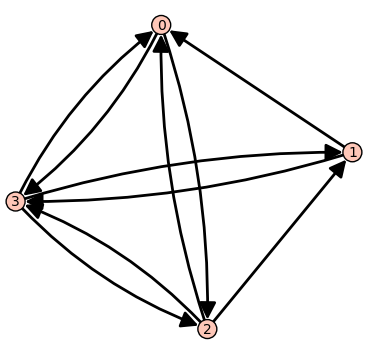
\includegraphics{graph_C.PNG} \\
    we choose
    $$C'=\begin{pmatrix}
    0 & 0 & 1 & 1\\
    1 & 0 & 1 &  0\\
    1 & 1 & 0 & 1\\
    1 & 1 & 1 & 0
    \end{pmatrix}.$$
    also, graph,\cite[sage]{sage}\\
    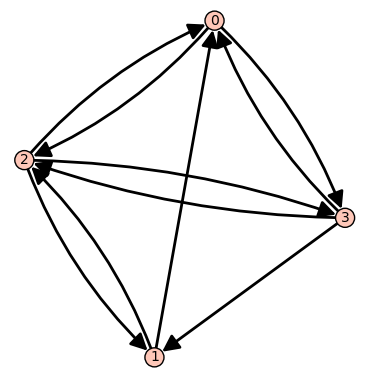
\includegraphics{graph_Cprime.PNG} \\
    Check the conditions $C[[n]|[n-1]]  \leq C'[[n]|[n-1]] $ of Theorem~\ref{thm_main},
    Then
    $\rho(C)\leq \rho(C')$ by previous Theorem~\ref{thm:conclusion}.



\subsection{Counterexample}
    For the following two $4\times 4$ matrices
    $$C=\begin{pmatrix}
    0 & 0 & 1 & 1\\
    1 & 0 & 0 & 1\\
    1 & 1 & 0 & 0\\
    1 & 1 & 1 & 0
    \end{pmatrix},\quad C'=\begin{pmatrix}
    0 & 0 & 1 & 1\\
    1 & 0 & 1 &  0\\
    1 & 1 & 0 & 0\\
    1 & 1 & 1 & 0
    \end{pmatrix},$$ 
    specify $n$=4, $k$=3 in $Q = I +E_{kn} = I + E_{34}$  
    $$CQ=\begin{pmatrix}
    0 & 0 & 1 & 2\\
    1 & 0 & 0 & 1\\
    1 & 1 & 0 & 0\\
    1 & 1 & 1 & 1
    \end{pmatrix},\quad C'Q=\begin{pmatrix}
    0 & 0 & 1 & 2\\
    1 & 0 & 1 & 1\\
    1 & 1 & 0 & 0\\
    1 & 1 & 1 & 1
    \end{pmatrix},$$

    we have $CQ\leq C'Q$, but 
    $\rho(C)=2.234\not\leq 2.148= \rho(C')$. 
    This is because $c'_{33}+c'_{34}\not\geq c'_{43}+c'_{44}$. 


    

%\section*{References}
\begin{thebibliography}{20}
\normalsize
\addcontentsline{toc}{section}{Bibliography}

\bibitem{chang}
Yen-Jen Cheng, {\it  A matrix realization of spectral bounds
of the spectral radius of a nonnegative matrix}, Ph.D. Thesis, NCTU, 2018.

\bibitem{spec_rad}
A. E. Brouwer, W. H. Haemers, {\it Spectra of graphs}, Springer, 2012

\bibitem{prn_fros2}
R. A. Horn , C. R. Johnson, {\it Matrix analysis}, Cambrigde University Press, 1985.

\bibitem{sage}
[Sage] SageMath, the Sage Mathematics Software System (Version 9.2),
       The Sage Developers, 2020, https://www.sagemath.org.  %sage tutorial

\end{thebibliography}




\end{document}
